\documentclass[runningheads]{llncs}
\usepackage[T1]{fontenc}
\usepackage[utf8]{inputenc}
\usepackage{minted}
\usemintedstyle{bw}
\setminted{fontsize=\small}

\usepackage{graphicx}

% *** CITATION PACKAGES ***
%
% \usepackage{cite}
%\renewcommand\cite[1]{[[#1]]}

\usepackage{hyperref}
\hypersetup{
    % bookmarks=true,         % show bookmarks bar?
    unicode=true,          % non-Latin characters in Acrobat’s bookmarks
    pdftoolbar=true,        % show Acrobat’s toolbar?
    pdfmenubar=true,        % show Acrobat’s menu?
    pdffitwindow=false,     % window fit to page when opened
    pdfstartview={FitH},    % fits the width of the page to the window
    %pdftitle={},    % title
    %pdfauthor={Author},     % author
    %pdfsubject={Subject},   % subject of the document
    %pdfcreator={Creator},   % creator of the document
    %pdfproducer={Producer}, % producer of the document
    %pdfkeywords={keyword1, key2, key3}, % list of keywords
    %pdfnewwindow=true,      % links in new PDF window
    colorlinks=true,       % false: boxed links; true: colored links
    linkcolor=black,          % color of internal links (change box color with linkbordercolor)
    citecolor=black,        % color of links to bibliography
    filecolor=black,      % color of file links
    urlcolor=black,           % color of external links
    final=true
  }




% *** GRAPHICS RELATED PACKAGES ***
%
% \ifCLASSINFOpdf
%   \usepackage[pdftex]{graphicx}
% \else
%   \usepackage[dvips]{graphicx}
% \fi





% *** MATH PACKAGES ***
%
%\usepackage[cmex10]{amsmath}



% *** ALIGNMENT PACKAGES ***
%
%\usepackage{array}


% *** SUBFIGURE PACKAGES ***
%\ifCLASSOPTIONcompsoc
%  \usepackage[caption=false,font=normalsize,labelfont=sf,textfont=sf]{subfig}
%\else
%  \usepackage[caption=false,font=footnotesize]{subfig}
%\fi


% correct bad hyphenation here
\hyphenation{op-tical net-works semi-conduc-tor}

%\providecommand\url[1]{\texttt{#1}}
\graphicspath{{pics/}}

\begin{document}
\urlstyle{tt}


\date{}
\title{Model Driven Architecture Implementation using Linked Data}

%\renewcommand\IEEEkeywordsname{Keywords}
%\DeclareRobustCommand*{\IEEEauthorrefmark}[1]{\raisebox{0pt}[0pt][0pt]{\textsuperscript{\footnotesize #1}}}
\author{%
  Evgeny Cherkashin\inst{1,2,5},
Alexey Kopaygorodsky\inst{3,5},
Ljubica Kazi\inst{4},
Alexey Shigarov\inst{1,2},
and
Vyacheslav Paramonov\inst{2}
}
%\authorrunning{E.~Cherkashin, A.~Kopaygorodsky, L.~Kazi et al.}
\institute{%
Irkutsk Scientific Center of SB RAS, 134 Lermontov Street, 664033, Russia \and
Matrosov Institute for System Dynamics and Control Theory of SB RAS, 134 Lermontov Street, 664033, Russia \and
Melentiev Energy Systems Institute of SB RAS, 130 Lermontov Street, 664033, Russia \and
University of Novi Sad, Technical faculty "Mihajlo Pupin", \DJ{}ure \DJ{}akovi\'ca bb,
 Zrenjanin, 23000, Serbia  \and
%Irkutsk State University, 20 Gagarina Avenue, 664002, Russia \and
National Research Irkutsk State Technical University, 83 Lermontov Street, 664074, Russia\\
\email{\href{mailto:eugeneai@icc.ru}{eugeneai@icc.ru},\href{mailto:digger@istu.edu}{digger@istu.edu},\href{mailto:ljubica.kazi@gmail.com}{ljubica.kazi@gmail.com}}%
}

% make the title area
\maketitle

\begin{abstract}
We consider tools for developing information systems with use of Model Driven Architecture (MDA) and Linked Open Data technologies (LOD).  The original idea of LOD is to allow the software designers to develop program systems integrated by means of common ontologies and web protocols.  MDA Platform Independent Model (PIM) is expressed as set of UML diagrams.  PIM forms a LOD graph and its namespace.  All the PIM entities are defined as ontology resources, \emph{i.e.} with URI references to LOD terms.  This allows us to translate PIM UML model to a set of triples and store them in an ontology warehouse for further transformation into a Platform Specific Model (PSM).  The ClioPatria ontology server and the SWI Prolog language are used as tools of PIM and PSM storage, querying and processing.
The tools will allow us to mediate the MDA static means of code generation and configuration at development stage with the techniques of flexible data structure processing at run time, thus, producing even more productive information system development and maintenance techniques.  This research corresponds to nowadays direction of Semantic Web Software Engineering.
\keywords{model driven architecture; linked open data; logic programming; knowledge based systems}
\end{abstract}

\section{Introduction}
% no \IEEEPARstart

Model Driven Architecture (MDA) is a software development methodology based on transformations of models of the software under development.  The input models are to be more abstract than generated output ones, as well as main aim of MDA is technological support of special cases of software development techniques.

Linked Open Data (LOD) \cite{Bizer} technology has been suggested by W3C consortium to represent the semantic information in the published web content in a way that provides not only the possibility of its processing with software agents (Semantic Web), but also to link all available information into a single semantic graph using relations and global universal identifiers (URIs) of resources. The descriptive capabilities of semantic web technologies, HTML5 document publishing tools, and LOD technologies form an infrastructural basis for, \emph{e.g.}, authoring and publishing documents \cite{Capadisli}. The LOD provide a logical markup for the information presented in a document, informative basis for the different variants of visual representation and interpretation, logical connections with other documents, export information into other documents, procedural processing, \emph{etc.} An important advantage of LOD usage in information environments is weakening of the requirements to the information warehouses: the document itself is a formalized data warehouse \cite{Cherk}. In some extent, this allows reallocation of the time spent on designing the database structure for storage of partially formalized documents to the process of solving a domain problem: the user (developer) markups the document text data with semantic meaning.

From the software designer point of view, LOD technologies allow development of program systems represent common and frequently used structures and data via common ontologies and web protocols \cite{Cherk}.  An application of semantic models at run time \cite{Kopay} allowed software designers to partially cope with problem of requirements and data structure evolution in lifespan of information systems.  A part of system configuration (static or dynamic) is build on domain ontology model interpretation, thus modifying information system behavior, resulting in a wider flexibility of system functioning.  LOD data can be used for description of various contexts and aspects, interface elements, their behavior, user access regulation, transactions, and so on.

We distinct four popular approaches of implementing Platform independent model (PIM) to Platform specific model (PSM) transformation, taking into account the runtime and other implementation platform features.  The first approach is model-to-model transformation with a model transformation language, such as QVT-X, ATL, \emph{etc.}  In this case PIM and resulting PSM are represented as XMI files.  Model transformation language rules recognizes structures in PIM and construct structures of PSM, having account various \texttt{boolean} conditions calculated with helper rules. The second variant of transformation is realized with Domain Specific Language (DSL) infrastructure \cite{stratego}.  The transformation procedure is presented as translation of one DSL instance, \emph{i.e.} PIM, to an instance in another language.

The third approach is a library-based one, it allows deigning the resulting PSM and the source code with functions from a library that are applied to predicates or complex structures as subtasks. Usage of interpreted or ahead-of-time-compilation languages as Python, Perl, PHP, ASP.NET, JavaScript, HTML as a target language for PSMs decreases the development time and make it less complex.  Thus, application of the libraries is the direct interaction of PIM as a superposition of applied function.  The fourth approach is the multistage transformation of the source PIM \cite{tereh1} on the base of logical inference.  The transformation is declared as a logical theory and a scenario of subgoals to be achieved.

The present research deals with developing software instrumental tools for general design of information systems using both Model Driven Architecture (MDA) and LOD \cite{MDA}.  MDA PIM is expressed as a set of UML diagrams (Class Diagram, State Diagram, \emph{etc.}) logically connected with rules of transformations.  PIM forms an RDF graph instance that can be assigned a namespace.  All the PIM elements are defined as A-Box ontology resources, \emph{i.e.} with URI references to LOD terms in a namespace of XMI standard.  The graph is stores in an ontology warehouse for further transformation into a PSM. %The stage of PIM design is very important as it in principle provides an evolution of the information system implementation within the development of the programming technologies in the future. %This means that correct and fully described PIM has more value versus PSM.
The ClioPatria ontology server and the SWI Prolog language \cite{Clio} are used as tools of PIM and PSM storage, querying and processing.

The direct way of a transformation implementation is to use \textsc{Prolog} or a functional language, and we use \textsc{Logtalk}, a macro package of Prolog.  The main advantage of the language usage is knowledge structuring thanks to its object-orientation.  Objects are used for representation of the source PIM model and the resulting PIM structures as well as source code generators.  Moreover, the transformation rules are easily integrated with libraries processing LOD and LOD warehouses.

The aim of this research is to construct tools for developing information systems with joint of MDA and LOD technologies in an indivisible cooperation.


\section{Related technologies and standards}
\label{sec:rel}

The most widely used technology of model transformation is ATL (ATLAS Transformation Language) \cite{atl} and its predecessor QVT, a OMG standard \cite{QVT}.  The language and its engine supports conversion from one XMI model to another one in the same format.  The language structures describe recognition of properties of compositions of the source model and direct construction of new structures in the target model accounting the property values.

The ATL is supported with visual tools for rule construction.  The tools are integrated in Eclipse IDE.  Similar to ATL, Transformation Model Representation Language (TMRL) is developed in \cite{nikita} but oriented on knowledge visual representation with following conversion in various production rules in CLIPS and OWL.  The visual presentation of transforming rules are used also in \cite{GT}, where a general approach is adopted for the purpose.  In a recent paper \cite{azis}, ATL is used to transform Computational Independent Model (CIM) represented as BPMN diagram into set of UML diagrams, defining PIM. Paper \cite{Rhazali} proposes a model transformation CIM to PIM for web-applications, where CIM is represented with State and Use case UML-Diagrams logically connected with ATL rules.  In \cite{Hamid} is proposed an evaluation of security aspects of distributed applications using MDA description; the evaluation is implemented a logical inference over the MDA synthesized logical security models. The paper \cite{Zdun} is considered a highly decoupled distributed event-driven application environment, whose design and functioning is dynamically controlled by its three-level DSL description and MDA transformations, which support change propagation.

Paper \cite{Malki} is presented a practical approach with four-level ATL-description from HTML-page to a LOD structure (via stage of an MDA PIM). In \cite{uml2owl}, a converter of UML package structures represented in XMI was developed as a XSLT transformation. A wide overview of Western approaches to program transformation is given in \cite{Dama,Dama2}, a transformation language PROMOL is suggested as well as its logical semantics. The book \cite{Dama}, together with John McCarthy's and Steve Russell's LISP technologies and Enn Tyugu's conceptual programming, covers the problem space history almost completely. OMG proposed ODM standard \cite{odmprof} for knowledge modeling.  A Visual Ontology Modeler \cite{odnext} is being developed for building and verifying OWL ontologies for ODM~1.0, as well as in the reverse direction, ontologies are represented as UML Class Diagrams \cite{odmvis}.

An XML based specifications are used in representing metadata about web services, WSDL \cite{wsdl}, and the WS-BPEL language \cite{wsbpel} for describing orchestration of web services within execution of an instance of a business process.  The idea of the language is to describe complex systems down to Web Services units, their internal and external structure and behavior, as well as services interaction in the script instance.

In our approach we use the structurally simplest language, Prolog, and its infrastructure, which is capable to load various model sources, including XMI, semantic graphs, \emph{etc.} with corresponding import module, as well as their processing \emph{em masse}, organizing multi-stage modular transformations. We also concentrate our efforts on programming in the small aspect of information system development, dealing with modeling and implementation software components composing software components.

\section{Transformation software architecture}
\label{sec:arch}

The architecture of the system is presented in Fig.~\ref{fig:arch}.  The PIM is designed with an UML editor as a set of diagrams.  We use Modelio \cite{modelio} as it contains means for formal definition of structured stereotypes, and it is open-sourced.  The model of an information system is converted in a RDF graph encapsulated in a Logtalk object.  The set of such objects are passed to the Transformation subsystem that is represented as a hierarchy of modules.  The subsystem queries server storage of ontologies and library rules stored on the server via Pengines interface module.  Library rules represent query helpers, which allow server-side preprocessing of the queries in its Inference machine.

\begin{figure}[t]
  \centering
  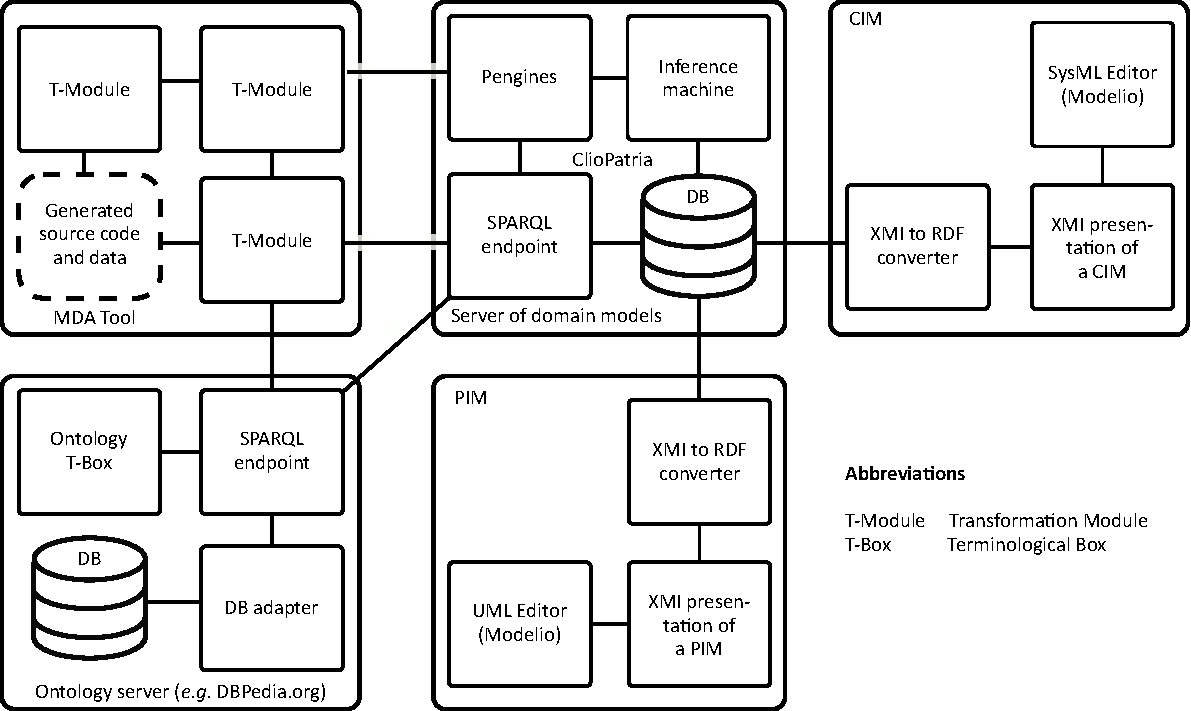
\includegraphics[width=1\linewidth]{architecture-mda-lod-ext.pdf}
  \caption{A general architecture of the PIM transformation system}
  \label{fig:arch}
\end{figure}

The server is being implemented on the base of ClioPatria ontology storage, which in turn is realized with SWI-Prolog programming system with some C language subroutines.  The ontology database supports durable storage and transactional querying as well as text search facility.  ClioPatria SPARQL queries execution subsystem operates in a federated regime out of the box.  The usage of Prolog based infrastructure for triple processing significantly reduces the structural and semantic complexity of whole system. It supports several formats of compact storage of RDF data.  The Pengines regulates access to the triples from clients, it is implemented as a simple protocol on top of HTTP.  %There are a number of implementation libraries for the protocols for popular programming languages, including client-side Prolog, JavaScript, Java, Python.

Ontologies are loaded into ClioPatria via its web interface, or by means of startup script with a library predicates.  ClioPatria has a simple interface for ontology browsing, transaction management, triple search by its literal values, and triple graph visualization for subset of triples.  The system has tools for SPARQL query testing and debugging.

\section{Implementation of transformation}
\label{sec:impl}

The transformation is implemented as a Logtalk library integrated with a RDF storage.  All the data processing is under control of SWI-Prolog.  No special DSL languages like ATL are needed, as we can do generalizations in LogTalk.  PIM logical structure is defined as a set of sources: UML-diagrams, ontologies and data stored in the warehouse of ontologies as well as other databases.  Logical connections of the elements of the sources are defined in a transformation program as well as the scenario of transformation.  The output of the transformation is a set of configured interlinked Logtalk objects representing PSM.  The source codes of the subsystems and the initial states of databases are generated from these object complexes.

At this stage of the research we implemented a processor of input XMI-2.0 files, which contain the UML-model of an information system, instances of transaction classes.  The XMI files exported by Modelio UML designer consist of a model of the system as a set of top packages, and two profile packages.  One profile package describes local definitions, and another represents the system and code generation configuration.  The import processor converts their DOM trees into corresponding graphs of RDF triples.  Each triple represents one relationship between two structural elements of an UML diagram.  The instances have public interface used to query their graphs for the structural element compositions.

Platform model (PM) in a broad sense is the transformation procedure implemented as Logtalk components (instances) organized in an hierarchy of transformation modules (Fig.~\ref{fig:modules}) in the image and likeness of our earlier work \cite{tereh1}.  Each component (module) queries the sources and constructs two classes of data: own state of private data and structures of external objects.  The states, in particular, contain type mappings between the source and target attributes, the implementation of designer decision on the general way of structure transformation.  %The Own states, in fact, represent the module configuration of its transformation state.

\begin{figure}[t]
  \centering
  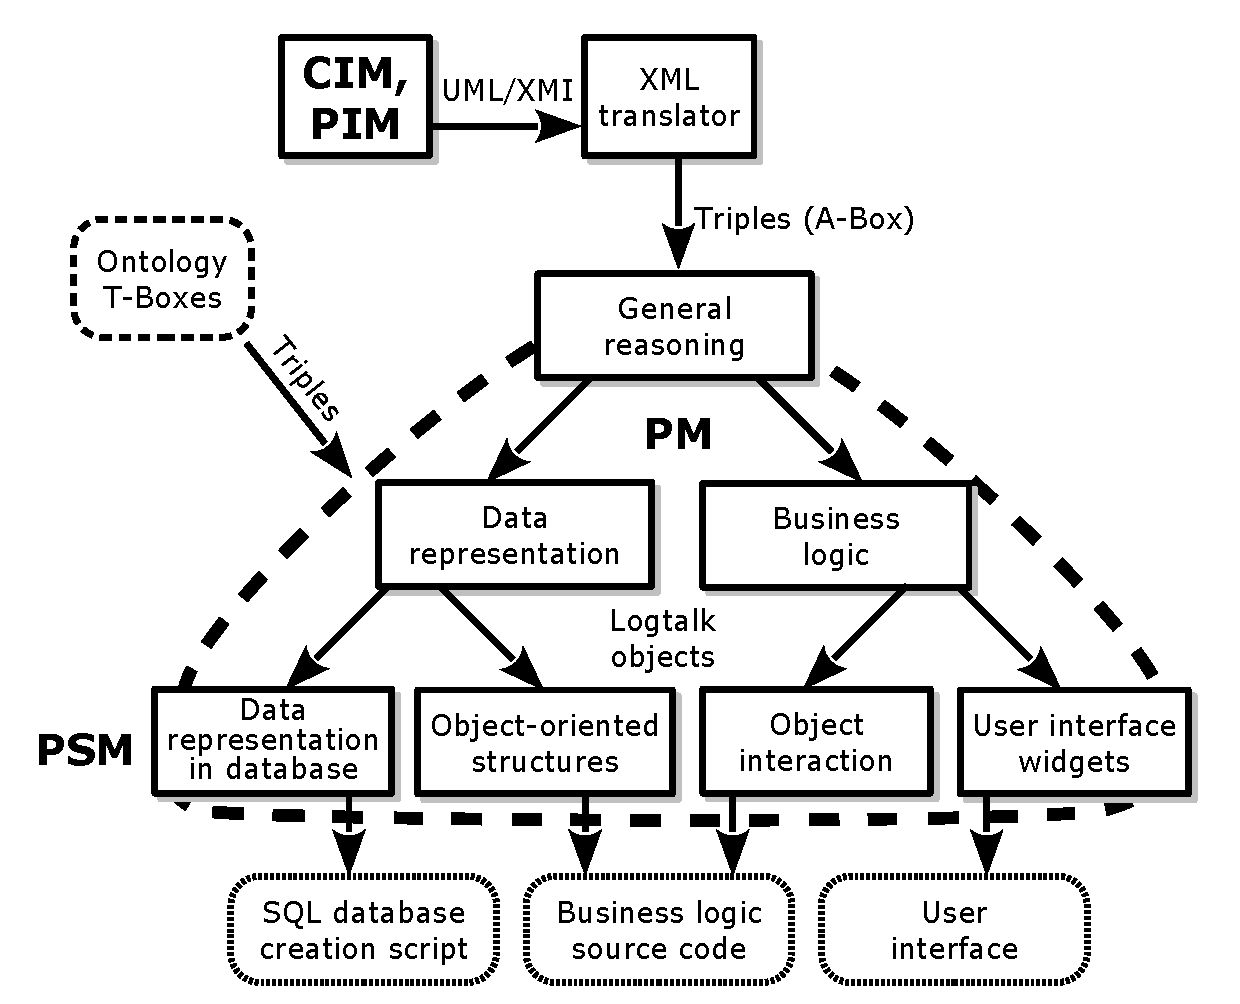
\includegraphics[width=1\linewidth]{architect_tree_pres-en-wo-OCL.pdf}
  \caption{A hierarchy of transformation modules representing PM}
  \label{fig:modules}
\end{figure}

External objects are structures constructing PSM, \emph{i.e.}, the set or a category of configured objects reflecting PIM structures and target sources and data.  Transformation modules generate the objects as a results of general decisions.  Their configurations are also inferred from the properties of structural elements of PIM and the profile configurations.  The leaf nodes of the hierarchy is the scenario of PSM generation.  The usage of pure logical approach instead of two languages allowed us to reduce the size and diversity of the PM description.

As soon as the scenario is fulfilled the PSM is converted into source codes and data.  The conversion in \cite{tereh1} was made by means of partial application of text templates.  In this case we do not use templates and generate the source code with simple procedures.  SWI-Prolong module index contains a simple template engine module \texttt{simple-template} intended for generation of static HTML pages.  The Prolog system also contain a dictionary-like structures and predicates for dictionary data manipulation, which can be used to represent data to be filled in the templates.  So open-source SWI-Prolog infrastructure is well equipped for developing MDA instruments.

\subsection{Inference of the class structure}
\label{sec:infstru}

Target class hierarchies in nowadays information system is diversified.  In web-applications, a PIM class or structure is mapped to a table or a SQL-query, an input form, an JavaScript object at user's browser, it can be a part of data transfer protocol like a JSON or XML object.  Some frameworks allow one to define structures and their relations and map them to rational databases, \emph{e.g.}, Django \cite{stratego} or Entity framework.  Most of the CASE-subsystems in UML composition tools do not support export of Class Diagram into ORM (Object-Relational Mapping) structures.

The main difference of MDA with respect to CASE technologies is the possibility of adaptation of PM to the special way of software development used in a particular software development group.  To put it on another way, MDA implements the standard transformations, and there is tools for modification of the standard procedures to implement own special techniques.  For example, if a programmer want to define a storage class for structures, the corresponding modification of standard transformation must be carried out.  Similarly a whole UML class hierarchy can be immersed into an ORM by means of a programmer-defined stereotype and its implementation.  Even an ORM itself may be implemented by means of special transformation.

\subsection{Inference of the properties}
\label{sec:infprop}

One of the interesting application of the Semantic WEB technologies, namely Linked Open Data, is the inference of the properties of the generated structural elements.  The properties of PSM elements, \emph{e.g.}, instance attributes, are derived from PIM UML structure elements, \emph{i.e.}, their standard UML definitions, analysis of relations being involved elements, features of combinations of associated stereotypes and tag values, as well as knowledge and data obtained from local ontology warehouse and SPARQL queries to other servers (cached for a better performance), for example, to \texttt{DBPedia.org}.

Consider the user interface template generation for a web or desktop application.  The model of the interface has a description of the structure and a specification of the properties of the constituent widgets.  If we refer from PIM with tag values \texttt{rdf:object} and \texttt{rdf:type} of a special stereotype \texttt{<<DBPedia>>} to a corresponding DBPedia resource we can use the DBPedia subgraph for constructing \texttt{title} and \texttt{placeholder} attributes of an input field.  In principle, we can figure out a label for user's locale.
%\subsection{Inference of methods}
%\label{sec:infmeth}
Some UML-structures (OCL) and relations may be interpreted constructively as methods of objects: events, handlers, subscribers, database triggers and selectors (lookups widgets).

% \begin{figure}[t]
%   \centering
%   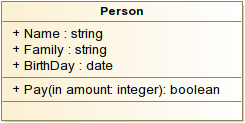
\includegraphics[width=0.6\linewidth]{pics/samples-Class-diagram.png}
%   \caption{A very simple Modelio PIM}
%   \label{fig:pim}
% \end{figure}

% \subsection{An example of simple transformation}
% \label{sec:simpletr}

Consider some transformation rules. In order to import PIM we need to create holding instance \texttt{sample} and initialize it. In this a very simple example. we represent a class \texttt{Person} in a Class diagram, server access code is omitted.
\begin{minted}{logtalk}
:- object(sample,instantiates(packageclass)).
:- initialization((::load_file('sample.xmi'),::reg_prefixes,::process)).
:- end_object.
\end{minted}
At the import stage, the source XMI converted into a graph.  We show its small part in the turtle format.
\begin{minted}{turtle}
@base <File://.../samples.xmi#>.
<#__k9i9BN_Eeijsfq5>
  a uml:Class;
  <#ownedAttribute> <#RN_Eeijsfq5>, <#hN_Eeijsfq5>, <#9xN_Eeijsfq5>;
  <#ownedOperation> <#BN_Eeijsfq5>; rdfs:label "Person".
<#__k9i9RN_Eeijsfq5>
  a uml:Property; <#type> <http://...#String>; <#visibility> "public";
  rdfs:label "Name".
<#BN_Eeijsfq5>
  a uml:Operation ;
  <#ownedParameter> <#hN_Eesfq5>, <#hN_Eesfq5>; <#visibility> "public";
  rdfs:label "Pay" .
\end{minted}

Construction of the target class is realized by querying the graph with a parametric object \texttt{query(\_Graph)}.
\begin{minted}{logtalk}
% ?- direct(sample,lp,cp)::tr(class,person,ID).
:- object(direct(_Package, _Local, _Code)).
tr(class, Class, ClassID):- ::package(Package), % obtain a PIM
  query(Package)::class(Name, ClassID),
  ::new(Class, [instantiates(class)]),
  ::new(Attributes,[instantiates(params)]),
  ::new(Methods, [instantiates(methodlist)]),
  Class::name(Name), % get class name.
  forall(::tr(attribute, Attribute, ClassID, _), % All attributes
      Attributes::append(Attribute)),
  forall(::tr(method, Method, ClassID,_), % All methods
      Methods::append(Method)),
  Class::attributes(Attributes), Class::methods(Methods). % construct
:- end_object.
:- object(query(_Graph)). % querying object
class(N, ID):- ::xmi(X), % the parameter N=Name, X=XMI
  X::rdf(ID, rdf:type, uml:'Class'), X::rdf(ID, rdfs:label, literal(N)).
:- end_object.
\end{minted}

Target structures constructed by blocks of elements and other blocks like in \texttt{llvmlite} library.  New \texttt{item}s are appended or prepended in a block.  Rendering the sources is realized with methods of construction classes.

\begin{minted}{logtalk}
:- object(class, specializes(code_block)).
renderitem(Item, Result):- ^^renderitem(Item, Result). % call parent.
render(Result):- ^^render(Name), .....
 root::indent, % Python block indentation
 (  ::item(attributes(Attributes))-> Attributes::render(DAttrs),
       root::iswritef(ConstructorDef, 'def __init__(self, %w):',[DAttrs]),
    root::indent, Attributes::items(InstAttrs),
    findall(S, (lists::member(Attr, InstAttrs), Attr::item(name(AttrName)),
                root::iswritef(S, "self.%w=%w", [AttrName, AttrName])),
            AttrAssigns), root::unindent,
    AttrList=[ConstructorDef|AttrAssigns];
    root::iswritef(ConstructorDef, 'def __init__(self):', []),
    root::indent, root::iswritef(Pass,'pass', []),
    root::unindent, AttrList=[ConstructorDef, Pass]    ),
   .....
  lists::append(AttrList, Methods, StringList), root::unindent,
  Result=[Signature | StringList]. % Join source lines.
:- end_object.
\end{minted}

As a result we obtain the following Python code.
\begin{minted}{python}
# ?- person::render_to(write).
class Person:
    def __init__(self, Name, Family, BirthDay):
        self.Name=Name
        self.Family=Family
        self.BirthDay=BirthDay
    def Pay(self, Amount):
        pass
\end{minted}

\section{Applications}
\label{sec:app}

The described MDA tools are used in a number of interesting projects.  The first project was to synthesize a Python interface driver of a cash register for a ticket system in a private cinema.

In the only Russian commercial planetary, a problem of connecting new cash register to a \emph{ad hoc} ticket and billing system arose.  The resources were limited by two weeks for main development and one programmer.  There was an old version of a program for the previous cash machine, a documentation to the new one, as well as test utility implementing the protocol obtained from vendor driver pack.  The description of the protocol in the manual was not precise: the sense of some fields were not understandable, the description of the automatons modeling the behavior in communications was too abstract, the documentation described two versions of the protocol, programmer has no experience related cash machines.

The decision of application of the MDA was made after the first investigation of the situation.  The protocol commands and the automatons were represented as UML Class and State diagrams.  After the application of the transformation adapted modules an interface component was generated.  The component encoded API call of a command into the bytes of protocol string and decoded the answer byte string from the cash machine into the answer object.  The interaction automaton of the computer and the cash device converted to a state machine with special states denoting exceptions related to undocumented and faulty behavior.  Tree levels of the interaction has been implemented: low-level protocol for message exchange, middle-level automaton cash machine state control and computer synchronization, and high-level algorithm implementing cash machine usage in fiscal operations within internet ticket booking system.

The low- and middle-level interaction were tested on dumped data of the test tool.  The tests showed the protocol documentation mistakes and version variant.  It also helped in PM and PIM refinement.  The first two levels of interaction started functioning in two weeks.  Another reserved two weeks was devoted to refinement of the fiscal operation, ticked printing design and deployment.

The second active project is a technological support of the development of New Generation Sequencing computation infrastructure for investigation of lake Baikal microbiome.  The investigation is a composition of elementary bioinfomatic operations implemented by external software like Mothur and R.  The developed tools are used to describe the operations as elements of a dataflow graph \cite{dataflow}.  Each operation communicates other ones with connections of ports.  The internal structures of its ports and parameters are represented with classes of UML Class Diagram.  The PM adopted to generate set of stub Java classes reflecting Mothur operations of Rapidminer Studio.  LOD is used to supply user descriptions in user interface for the operations.

%FIXME: Extend here till fill of 12th page.

% \subsection{Future projects}
% \label{sec:futuretargets}

% The LOD technologies will be used in development of an extension module for Electronic Medical Record (EMR) subsystem in Irkutsk Regional Oncological Dispancery.  The aim of development is to incorporate into the diagnosis texts a markup that can be used in expert decision-making procedures, \emph{e.g.}, for quality control.

% A patient must be specially prepared for surgery: a set of tests must be taken, the tests must correspond to criteria, the patient must be properly hospitalized, special preparatory procedures must be carried out, \emph{etc.}  All results are filled in check lists.   If patient's check list satisfies the conditions the patient is allowed to be surgically operated.  After the surgery a set of new manipulations are to be carried out.

% The stated development is the very place for our MDA tools and LOD technologies application.  The EMR text field of the test results and diagnoses is used to store semiformalized representation of the input data for check lists.  The EMRs are divided into classes (types), and we can associate the type and its text LOD markup template.  The set of the attributes for each type is defined as classes of UML Class Diagram.  Check lists and set of after-surgery operation are represented as classes as well.  The input, check list, and new operations are joined in a special relation forming templates describing one quality control and planing module.

% Thus, the usage of MDA in this task will allow incremental improvement of the quality control by means of visual construction of the templates.  Using LOD allows us to develop the main EMR, and the quality control and planning subsystems absolutely independently, effectively hiding complex behavior of EMR texts from main middle-ware and database structures.  It simplifies also the structure of the main database.

% Another interesting project is a development of a recommender system for the Irkutsk region real estate market.  The aim is to implement user means for assisting in decision making and choice refinement.  The real estate objects (flats, houses, offices) have various attributes, which used to describe the objects.  Each type of the objects are to be represented as classes in PIM, as well as the features of the user.

% The attributes, features, and their relation constructed on the base of a domain ontology are the basis of logical processing of the database data and measuring the user interest to the object.  In this case the transformation modules convert the input XMI-data into a subgraph of A-box of Irkutsk region real estate domain ontology and into interface classes describing entities of BrightstarDB object-RDF mapping database.  The LOD is added as resource references to the external ontologies and individual resources.  Thus, in this case the MDA tools are used as ontology modeling software.

\section{Conclusion}

We considered an implementation and applications of usage of Model Driven Architecture and Linked Open Data, a Semantic Web, technologies in developing software \cite{SWEB} on the base of model transformation.  The transformation is realized as a hierarchy of objects represented in LogTalk.  Results of analysis of the source model and synthesis of the target one are obtained with logical inference.

Usage of logical programming language simplifies the transformation procedure programming, the programmer is allowed to express semantics of recognized structures as properties of objects, manipulate object properties further. It also allows us to integrate the transformations with other Prolog libraries and services without usage of special language structures. The transformation logically connect elements of source objects: UML diagrams, RDF A- and T-boxes, LogTalk modules, which are just structures to be processed accounting to a scenario.

The approach is being tested in software development processes for synthesis of business-objects of information systems carcasses, interface modules for a protocol, as an ontology development tool, \emph{etc.} Further development of the software is aimed at extending transformation modules, creating libraries of platform descriptions for open-source frameworks, develop techniques of change propagation, and developing open-source UML editors to support UML~2.5 profile specification \cite{uml25} and XMI export.

% One of the problem of tools construction of such kind is the absence of visual editors of UML supporting ontology models.  The UML 2.4 standard implicitly suggests coupling stereotypes and tag values forming a data format representing stereotype aspects of the UML entities.  Thus, one of the research direction is to construct new or adapt existing UML modeling tool to support LOD in UML diagrams.
% At the time moment of the paper submission the \texttt{Modelio} tool did not support export stereotype structures described in so called profiles of the PIM.  We emulate their export manually.  Other open-source tools like \texttt{ArgoUML}, BoUML, Papyrus, Umlet, \emph{etc.} either too far from the stereotype support or too complex in user interface or do not export the PIM as XMI-file.

\section*{Acknowledgment}

The results are obtained with the partial support of the various projects: Irkutsk scientific center of SB RAS No 4.2;
The Council for grants of the President of Russian Federation, state support of leading scientific schools of the Russian Federation (NSH-8081.2016.9); Russian Foundation for Basic Research, grants 17-07-01341, 18-07-00758 and 17-47-380007. The results obtained with the use of the network infrastructure of Telecommunication center of collective use "Integrated information-computational network of Irkutsk scientific-educational complex" (\url{http://net.icc.ru}). The authors are grateful to the community of Linked Open Vocabularies (\url{http://lov.okfn.org/dataset/lov/}) resource for assistance in the search for domain ontologies and \texttt{github.com} for hosting sources at \url{https://github.com/isu-enterprise/icc.xmitransform}.

\begin{thebibliography}{11}
\bibitem{Bizer} \textbf{Ch.\,Bizer, T.\,Heath, T.\,Berners-Lee.} Linked Data -- The Story So Far. \emph{Semantic Web and Information Systems}. 2009. Vol. 5 (3). pp.~1--22.
\bibitem{Capadisli} \textbf{S.\,Capadisli, A.\,Guy, R.\,Verborgh, C.\,Lange, S.\,Auer, T.\,Berners-Lee.} Decentralised Authoring, Annotations and Notifications for a Read-Write Web with dokieli, In: Cabot J., De Virgilio R., Torlone R. (eds) \emph{Web Engineering. ICWE 2017. Lecture Notes in Computer Science.} vol 10360. Springer, Cham. Preprint URL:\url{http://csarven.ca/dokieli-rww}, DOI:\url{10.1007/978-3-319-60131-1_33}.
\bibitem{Cherk} \textbf{E.\,Cherkashin, I.\,Orlova.} Instrumental tools for construction of the digital archives of the documents based on Linked Data. \emph{Modern technologies, System analysis, Modeling.} 4(56) 2017 pp. 100-107 (in Russian) \href{http://stsam.irgups.ru/sites/default/files/articles\_pdf\_files/100-107.pdf}{doi:10.26731/1813-9108.2017.4(56).100-107}
\bibitem{Kopay} \textbf{A.\,Kopaygorodsky.} Use of ontologies in semantic information systems. \emph{Ontology of Design.} vol.~4(14), 2014, pp.~78--89 (in Russian) %URL:\href{http://agora.guru.ru/scientific_journal/files/Ontology_Of_Designing_4_2014_opt1.pdf#page=79}{\ttfamily %http://agora.guru.ru/scientific\_journal/files/On\-tology\_Of\_Designing\_4\_2014\_opt1.pdf}
\bibitem{stratego} \textbf{D.\,Annenkov, E.\,Cherkashin.} Generation Technique for Django MVC Web Framework Using the Stratego Transformation Language. \emph{Proc. of 36th International Convention on Information and Communication Technology, Electronics and Microelectronics (MIPRO).} May 20--24, 2013, Opatija, Croatia, 2013, pp.~1084--1087.
\bibitem{tereh1} \textbf{E.\,Cherkashin, A.\,Larionov et al.} Logical programming and data mining as engine for MDA model transformation implementation. \emph{Procs of 36th International Convention on Information and Communication Technology, Electronics and Microelectronics (MIPRO).} May 20--24, 2013, Opatija, Croatia, pp.~1029--1036.
\bibitem{MDA} \textbf{D.\,Frankel.} Model Driven Architecture: Applying MDA to Enterprise Computing. Wiley; 1 edition, 2003, 352 p.
\bibitem{Clio} \textbf{J.\,Wielemaker, W.\,Beek, M.\,Hildebrand, J.\,Ossenbruggen.} ClioPatria: A SWI-Prolog Infrastructure for the Semantic Web, \emph{Semantic Web.} vol. 7, no. 5, 2016, pp.~529-541. DOI:\url{10.3233/SW-150191}
\bibitem{atl} \textbf{F.\,Jouault, F.\,Allilaire, J.\,Bezivin, I.\,Kurtev.} Atl: A model transformation tool. \emph{Sci. Comput. Program.} 72(1--2), pp.~31--39 (2008)
\bibitem{QVT} The MOF Query/View/Transformation Specification Version 1.1. URL:\url{http://www.omg.org/spec/QVT/1.1}
\bibitem{nikita} \textbf{A.\,Berman, M.\,Grishchenko, N.\,Dorodnykh, O.\,Nikolaychuk, A.\,Yurin.} A model-driven approach and a tool to support creation of rule-based expert systems for industrial safety expertise. \emph{Proc. of the 12 th International Forum on Knowledge Asset Dynamics (IFKAD-2017)} -- Russia, St.\,Petersburg : Graduate School of 16 Management of St.\,Petersburg University.  2017.  P.~2034--2050.
\bibitem{GT} \textbf{A.\,Belghiat, M.\,Bourahla.} UML Class Diagrams to OWL Ontologies: A Graph Transformation based Approach. \emph{International Journal of Computer Applications}. 41. pp.~41--46. 10.5120/5525-7566.
\bibitem{azis}\textbf{Y.\,Rhazali, Y.\,Hadi, A.\,Mouloudi.} Model Transformation with ATL into MDA from CIM to PIM Structured through MVC. \emph{Procedia Computer Science 83} (2016) 1096–1101. URL:\url{https://doi.org/10.1016/j.procs.2016.04.229}
\bibitem{Rhazali}
\textbf{Y.\,Rhazali, Y.\,Hadi, I.\,Chana, M.\,Lahmer, A.\,Rhattoy.} A model
transformation in model driven architecture from business model to web
model. \emph{IAENG International Journal of Computer Science}, vol.~45(1), 2018, 104-117, URL:\url{http://www.iaeng.org/IJCS/issues_v45/issue_1/IJCS_45_1_16.pdf}.
% The paper \ref{Rhazali} proposes a model  transformation  method  to  master  the  transformation
% from  CIM  to  PIM  web-based  in  accordance  with  the  Model
% Driven  Architecture  approach. CIM is represented mainly with State and Use case UML-Diagrams connected with ATL rules.

\bibitem{Hamid}
\textbf{B.\,Hamid, D.\,Weber.} Engineering secure systems: Models, patterns
and empirical validation. \emph{Computers \& Security},  vol~77, 2018, p.~315-348.
\href{https://www.sciencedirect.com/science/article/pii/S0167404818303043}{doi:10.1016/j.cose.2018.03.016}

% In \ref{Hamid} an approach proposed for evaluation security aspects of distributed applications using modeling, MDA description and synthesis of the applications. A logical inference evaluation is carried out over the MDA synthesized logical security models.

\bibitem{Zdun}
\textbf{S.\,Tragatschnig, S.\,Stevanetic, U.\,Zdun.} \href{https://www.sciencedirect.com/science/article/abs/pii/S0950584916303251}{Supporting the
evolution of event-driven service-oriented architectures using change
patterns.} \emph{Information and Software Technology.} vol.~100, 2018, p.~133-146. \href{doi:10.1016/j.infsof.2018.04.005}{https://www.sciencedirect.com/science/article/abs/pii/S0950584916303251}


% The paper \ref{Zdun} is considered a highly decoupled distributed event-driven application environment, whose design and functioning is dynamically controlled by its three-level DSL description and MDA transformations, which support change propagation.

\bibitem{Malki}
\textbf{B.\,Bouougada, D.\,Bouchiha, M.\,Malki} A framework for
reengineering web applications into linked data based on MDA. Paper
presented at the ACM International Conference Proceeding Series, 2015,
23-25-November-2015 doi:10.1145/2816839.2816880

% In \ref{Malki} a practical approach implemented with four-level description of ATL transformations from HTML-page to a RDF structure (via stage of an MDA PIM), which represents HTML (LI,TABLE, etc.) data as LOD.

\bibitem{uml2owl} UMLtoOWL: Converter from UML to OWL. URL: \url{http://www.sfu.ca/~dgasevic/projects/UMLtoOWL/}.
\bibitem{Dama}
\textbf{V.\,\v{S}tuikys, R.\,Dama\v{s}evi\v{c}ius.} Meta-program development as a
model transformation process. 2013. doi:10.1007/978-1-4471-4126-6\_11
% A wide overview of Western approaches to program transformation is given in \cite{Dama,Dama2}, the language PROMOL is suggested as well as its logical semantics. The book \cite{Dama}, together with John McCarthy's and Steve Russell's LISP technologies and Enn Tyugu's conceptual programming, covers the problem space history almost completely.

\bibitem{Dama2}
\textbf{V.\,\v{S}tuikys, R.\,Dama\v{s}evi\v{c}ius, A.\,Targamadze.} A model-driven
view to meta-program development process. \emph{Information Technology and
Control.} vol.~39(2), 2010, p.~89-99. URL:\url{http://itc.ktu.lt/index.php/ITC/article/download/12302/6838}
\bibitem{odmprof} ODM UML profile for OWL. URL:\url{http://www.omg.org/spec/ODM/1.0/PDF/}.
\bibitem{odnext} Ontology Domain Modeling example. URL:\url{https://thematix.com/tools/vom/}.
\bibitem{odmvis} OWL UML Visualizer. URL:\url{http://owlgred.lumii.lv/}.
\bibitem{wsdl} Web Services Description Language -- Wikipedia, the free encyclopedia.  URL:\url{https://en.wikipedia.org/wiki/Web_Services_Description_Language}
\bibitem{wsbpel} Business Process Execution Language -- Wikipedia, the free encyclopedia. \url{https://en.wikipedia.org/wiki/Business_Process_Execution_Language}
\bibitem{modelio} Modelio Open Source -- UML and BPMN free modeling tool. URL:\url{https://www.modelio.org/}.
\bibitem{dataflow} \textbf{Johnston W.M., Hanna J.R.P., Millar R.J.} Advances in Dataflow Programming Languages.
  \emph{ACM Computing Surveys}. -- 2004. -- Vol. 36. -- pp. 1--34.
  2004.~--~Vol.~36.~--~P.~1--34.
\bibitem{SWEB} Semantic WEB Software Engineering. URL:\url{http://www.webist.org/Documents/Previous\_Invited\_Speakers/2012/WEBIST2012\_Pan.pdf}. %URL:\url{https://www.iospress.nl/book/semantic-web-enabled-software-engineering/}.
\bibitem{uml25} Unified Modeling Language, ver.~2.5 standard description. URL:\url{http://www.omg.org/spec/UML/2.5/PDF}



\end{thebibliography}




% that's all folks
\end{document}

%%% Local Variables:
%%% TeX-master: t
%%% End:
